% Generated from the public primitive catalog. Original Atlas drawing; Apache-2.0.
% Target: md5; view: overview-compact
\documentclass[border=9pt]{standalone}
% Original Atlas figure theme. Apache-2.0; see the repository LICENSE.
\usepackage[T1]{fontenc}
\usepackage{lmodern}
\usepackage{amsmath,amssymb}
\usepackage{tikz}
\usetikzlibrary{arrows.meta,positioning,calc,fit,backgrounds,decorations.pathreplacing,matrix}
\definecolor{atlasInk}{HTML}{172235}
\definecolor{atlasTeal}{HTML}{0D7B7D}
\definecolor{atlasMuted}{HTML}{637278}
\definecolor{atlasFill}{HTML}{EAF4F2}
\definecolor{atlasLine}{HTML}{B6C8C7}
\tikzset{
  every picture/.style={line width=.65pt,draw=atlasInk,>=Latex},
  every node/.style={text=atlasInk,font=\sffamily\small},
  box/.style={draw,rounded corners=1.5pt,minimum height=.9cm,minimum width=1.6cm,align=center,inner sep=6pt,fill=white},
  accent/.style={box,draw=atlasTeal,fill=atlasFill},
  wire/.style={->,line width=.7pt},
  keywire/.style={wire,draw=atlasTeal,dashed},
  xor/.style={draw,circle,fill=white,inner sep=0pt,minimum size=.38cm},
  add/.style={draw,rectangle,fill=white,inner sep=0pt,minimum size=.38cm},
  note/.style={font=\sffamily\scriptsize,text=atlasMuted,align=center},
  phase/.style={font=\sffamily\small\bfseries,text=atlasTeal},
  group/.style={draw=atlasLine,dashed,rounded corners=2pt,inner sep=8pt}
}
\newcommand{\rotl}{\mathbin{\lll}}
\newcommand{\rotr}{\mathbin{\ggg}}
\newcommand{\kx}{\operatorname{Keccak}\!\text{-}\!f[1600]}

\newcommand{\AtlasKeyBits}{k}
\newcommand{\AtlasKeyWords}{N_k}
\newcommand{\AtlasRounds}{N_r}
\newcommand{\AtlasPriorRounds}{N_r-1}
\newcommand{\AtlasRoundKeys}{N_r+1}
\newcommand{\AtlasDoubleRounds}{N_r/2}
\newcommand{\AtlasSixRoundGroups}{N_r/6}
\newcommand{\AtlasFLGroups}{N_r/6-1}
\newcommand{\AtlasRoundStart}{24-n}
\newcommand{\AtlasBlockBits}{512}
\newcommand{\AtlasOutputBits}{128}
\newcommand{\AtlasStateBits}{128}
\newcommand{\AtlasNonceBits}{v}
\newcommand{\AtlasCounterBits}{q}
\newcommand{\AtlasStreamBlockBits}{b}
\newcommand{\AtlasRate}{r}
\newcommand{\AtlasCapacity}{c}
\newcommand{\AtlasSteps}{64}
\newcommand{\AtlasLastStep}{63}
\newcommand{\AtlasWordBits}{16}
\newcommand{\AtlasHashWords}{4}
\newcommand{\AtlasFeedForward}{\boxplus}
\newcommand{\AtlasByteOrder}{little-endian}
\newcommand{\AtlasDomain}{01}
\newif\ifAtlasXof
\AtlasXoffalse
\begin{document}
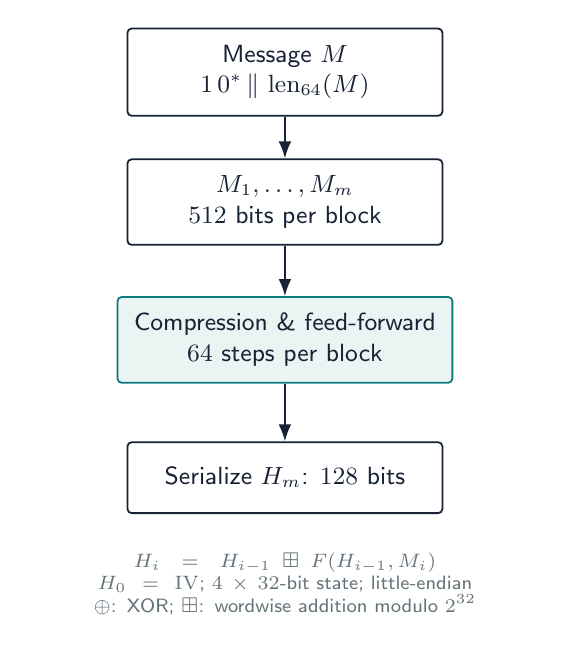
\begin{tikzpicture}
  \node[box,minimum width=4cm] (pad) at (0,0) {Message $M$\\$1\,0^*\,\|\,\operatorname{len}_{64}(M)$};
  \node[box,minimum width=4cm] (blocks) at (0,-1.65) {$M_1,\ldots,M_m$\\$\AtlasBlockBits$ bits per block};
  \node[accent,minimum width=4cm] (compress) at (0,-3.4) {Compression \& feed-forward\\$\AtlasSteps$ steps per block};
  \node[box,minimum width=4cm] (out) at (0,-5.15) {Serialize $H_m$: $\AtlasOutputBits$ bits};
  \draw[wire] (pad) -- (blocks); \draw[wire] (blocks) -- (compress); \draw[wire] (compress) -- (out);
  \node[note,text width=6.3cm] at (0,-6.5) {$H_i=H_{i-1}\AtlasFeedForward F(H_{i-1},M_i)$\\$H_0=\mathrm{IV}$; $\AtlasHashWords\times32$-bit state; \AtlasByteOrder\\$\oplus$: XOR; $\boxplus$: wordwise addition modulo $2^{32}$};
\end{tikzpicture}

\end{document}
